\begin{frame}{Tổng quan các phương pháp phát hiện té ngã}
\scriptsize
\begin{tabular}{|p{0.18\linewidth}|p{0.22\linewidth}|p{0.25\linewidth}|p{0.25\linewidth}|}
\hline
\textbf{Phương pháp} & \textbf{Cơ chế} & \textbf{Ưu điểm} & \textbf{Nhược điểm} \\
\hline
Đeo được & IMU (gia tốc kế, con quay hồi chuyển); phát hiện gia tốc/tư thế bất thường & Phản hồi nhanh; chính xác; chi phí thấp & Cần đeo liên tục; dễ false positive; pin/hiệu chuẩn \\
\hline
Môi trường & Cảm biến cố định: sàn áp suất, PIR, âm thanh; AI phân tích & Không xâm phạm; giám sát nhiều người; tích hợp smart home & Chi phí cao; phạm vi hạn chế; nhầm vật thể \\
\hline
Thị giác & Camera RGB/RGB-D/IR; pose estimation (OpenPose/MediaPipe) & Thông tin trực quan; không cần đeo; tích hợp giám sát & Quyền riêng tư; phụ thuộc ánh sáng; cần phần cứng mạnh \\
\hline
Đa phương thức & Kết hợp IMU + camera + môi trường; data fusion (Kalman/Deep Learning) & Độ chính xác cao; giảm cảnh báo sai; mở rộng phạm vi; kinh tế & Phức tạp; tốn năng lượng; đồng bộ khó \\
\hline
\end{tabular}

\vspace{0.3em}
\begin{itemize}\scriptsize
    \item Kết hợp dữ liệu để xác nhận té ngã, giảm false positive.  
    \item Chế độ linh hoạt: In-situ (cục bộ) + Mobile (edge device).  
    \item Bảo mật: xử lý cục bộ, chỉ gửi dữ liệu tối thiểu, tùy chỉnh khu vực nhạy cảm.
\end{itemize}
\end{frame}
% Slide 1: Tổng quan
\begin{frame}
\frametitle{Các Giao Thức Truyền Thông trong Hệ Thống Cảnh Báo IoT}
\begin{center}
\Large Hệ thống phát hiện ngã với ba giao thức cốt lõi
\end{center}

\begin{itemize}
\item \textbf{SIP}: Truyền tải âm thanh/video cảnh báo thời gian thực
\item \textbf{MQTT}: Vận chuyển dữ liệu cảm biến từ thiết bị IoT  
\item \textbf{JSON}: Định dạng cấu trúc dữ liệu trao đổi
\end{itemize}

\begin{block}{Mục tiêu}
Xây dựng hệ thống cảnh báo không gián đoạn, độ trễ thấp từ cảm biến đến cuộc gọi VoIP
\end{block}
\end{frame}

% Slide 2: Giao thức SIP
\begin{frame}
\frametitle{Giao thức SIP - Khởi tạo Phiên}

\textbf{Chức năng chính:}
\begin{itemize}
\item Thiết lập cuộc gọi VoIP từ hệ thống cảnh báo
\item Kết nối với Asterisk PBX để gọi điện thoại
\item Truyền âm thanh cảnh báo qua RTP
\end{itemize}

\textbf{Các bước hoạt động:}
\begin{enumerate}
\item REGISTER: Đăng ký thiết bị với server
\item INVITE: Khởi tạo cuộc gọi cảnh báo
\item ACK: Xác nhận kết nối thành công
\item RTP: Truyền dữ liệu âm thanh
\item BYE: Kết thúc cuộc gọi
\end{enumerate}

\begin{alertblock}{Lưu ý}
Sử dụng ICE để xuyên NAT, TLS/SRTP để bảo mật
\end{alertblock}
\end{frame}

% Slide 3: Giao thức MQTT
\begin{frame}
\frametitle{Giao thức MQTT - Truyền Dữ Liệu Cảm Biến}

\textbf{Đặc điểm:}
\begin{itemize}
\item Nhẹ, tiết kiệm băng thông cho thiết bị IoT
\item Mô hình Publish/Subscribe qua Broker
\item Hỗ trợ 3 mức QoS đảm bảo độ tin cậy
\end{itemize}

\textbf{Mức QoS:}
\begin{itemize}
\item \textcolor{green}{\textbf{QoS 0}}: Gửi một lần (dữ liệu thường)
\item \textcolor{orange}{\textbf{QoS 1}}: Ít nhất một lần (có xác nhận)
\item \textcolor{red}{\textbf{QoS 2}}: Đúng một lần (cảnh báo quan trọng)
\end{itemize}

\textbf{Ví dụ topic:} \texttt{sensor/room/temperature}, \texttt{alert/fall/detected}
\end{frame}

% Slide 4: JSON và Tích hợp Hệ thống
\begin{frame}
\frametitle{JSON và Tích Hợp Hệ Thống}

\textbf{JSON - Định dạng dữ liệu:}
\begin{itemize}
\item Nhẹ, dễ đọc, tương thích đa nền tảng
\item Cấu hình thiết bị và trao đổi dữ liệu cảm biến
\item Tối ưu payload cho MQTT
\end{itemize}

\textbf{Luồng tích hợp hoàn chỉnh:}
\begin{enumerate}
\item ESP32 phát hiện ngã → tạo JSON payload
\item Gửi qua MQTT topic với QoS phù hợp  
\item Ứng dụng trung gian nhận và xử lý JSON
\item Kích hoạt cuộc gọi SIP qua Asterisk AMI
\item Phát cảnh báo âm thanh đến điện thoại
\end{enumerate}
\end{frame}

% Slide 5: Kết luận và Tối ưu
\begin{frame}
\frametitle{Kết Luận và Tối Ưu Hóa}

\textbf{Lợi ích của việc kết hợp 3 giao thức:}
\begin{itemize}
\item \textbf{MQTT}: Thu thập dữ liệu hiệu quả từ cảm biến
\item \textbf{JSON}: Cấu trúc dữ liệu linh hoạt, dễ xử lý
\item \textbf{SIP}: Cảnh báo âm thanh tức thì, đáng tin cậy
\end{itemize}

\textbf{Các biện pháp tối ưu:}
\begin{itemize}
\item Payload JSON nhỏ gọn tiết kiệm năng lượng
\item QoS MQTT phù hợp với mức độ quan trọng
\item Tự động kết nối lại khi mất kết nối
\item Bảo mật TLS cho MQTT và SIP
\end{itemize}

\begin{block}{Kết quả}
Hệ thống cảnh báo tự động, tin cậy từ thiết bị nhúng đến cuộc gọi VoIP
\end{block}
\end{frame}

%mdeida pose edge----------------- edge
\begin{frame}
\frametitle{Hình ảnh An toàn}
\begin{columns}
\begin{column}{0.4\textwidth}
    \begin{figure}
    \centering
    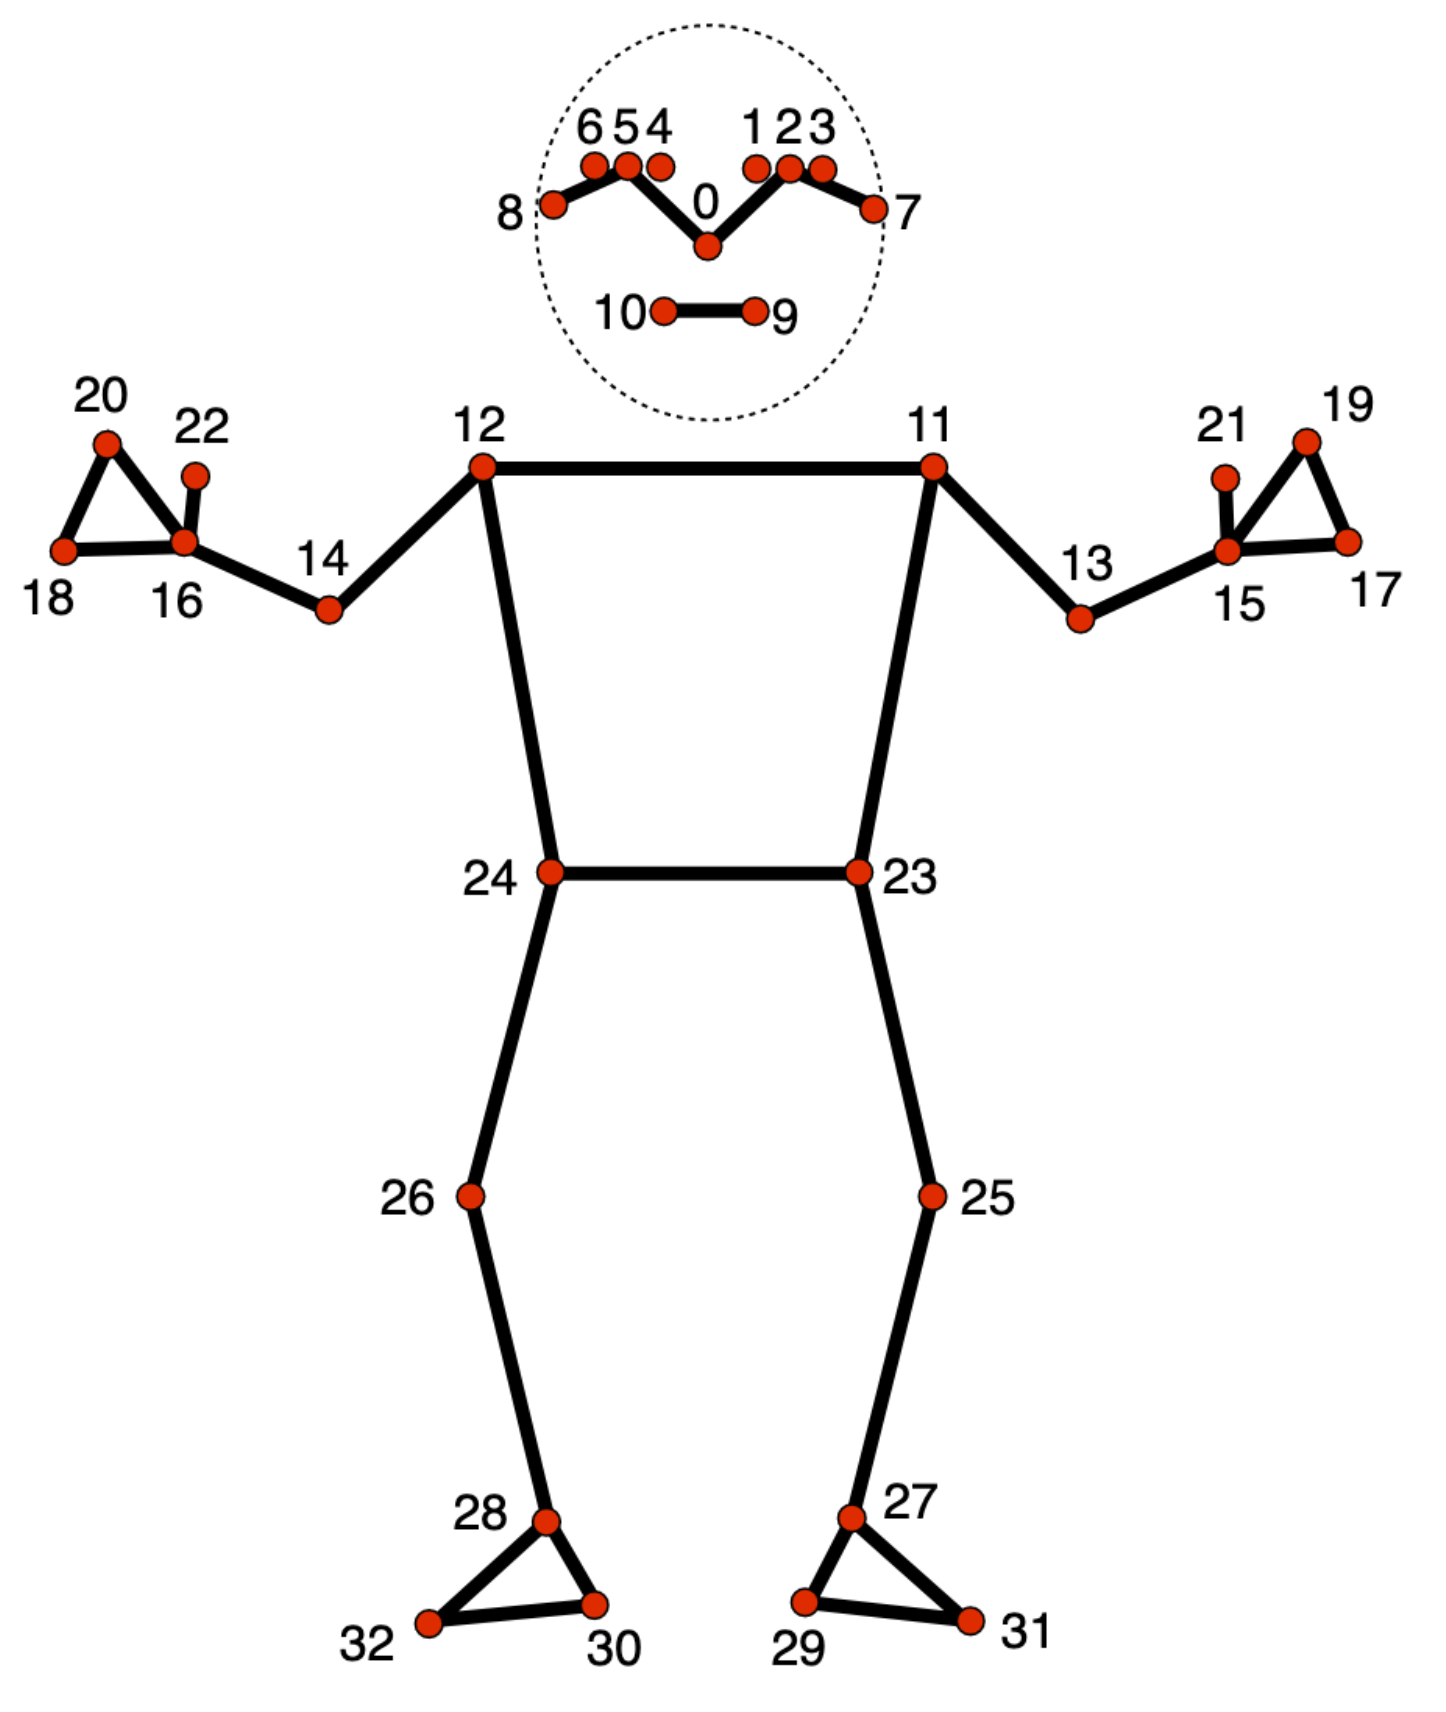
\includegraphics[width=\textwidth]{pose_landmarks_index.png}
    \caption{Hình ảnh mô tả.}
    \end{figure}
\end{column}
\begin{column}{0.6\textwidth}
    \begin{block}{Mô tả Chi tiết}
    Sử dụng \textbf{MediaPipe} là giải pháp then chốt để có được các điểm mốc 3D chính xác.
    \end{block}
\end{column}
\end{columns}
\end{frame}

%mdeida pose edge----------------------------yy------------------- edge

% Slide 1: Section Overview
\begin{frame}{Nhận diện Tư thế Người và Phát hiện Té ngã}
    \begin{block}{Tổng quan}
        Hệ thống tích hợp nhận diện tư thế (MediaPipe Pose) và phát hiện té ngã dựa trên đặc trưng động học/tư thế.
        \begin{itemize}
            \item Ứng dụng: Giám sát an toàn, phát hiện té ngã.
            \item Nền tảng: Thị giác máy tính thời gian thực.
        \end{itemize}
    \end{block}
\end{frame}


\begin{frame}{Nhận diện Tư thế Người}
\begin{columns}[T]
    % Column Hình
    \begin{column}{0.45\textwidth}
        \centering
        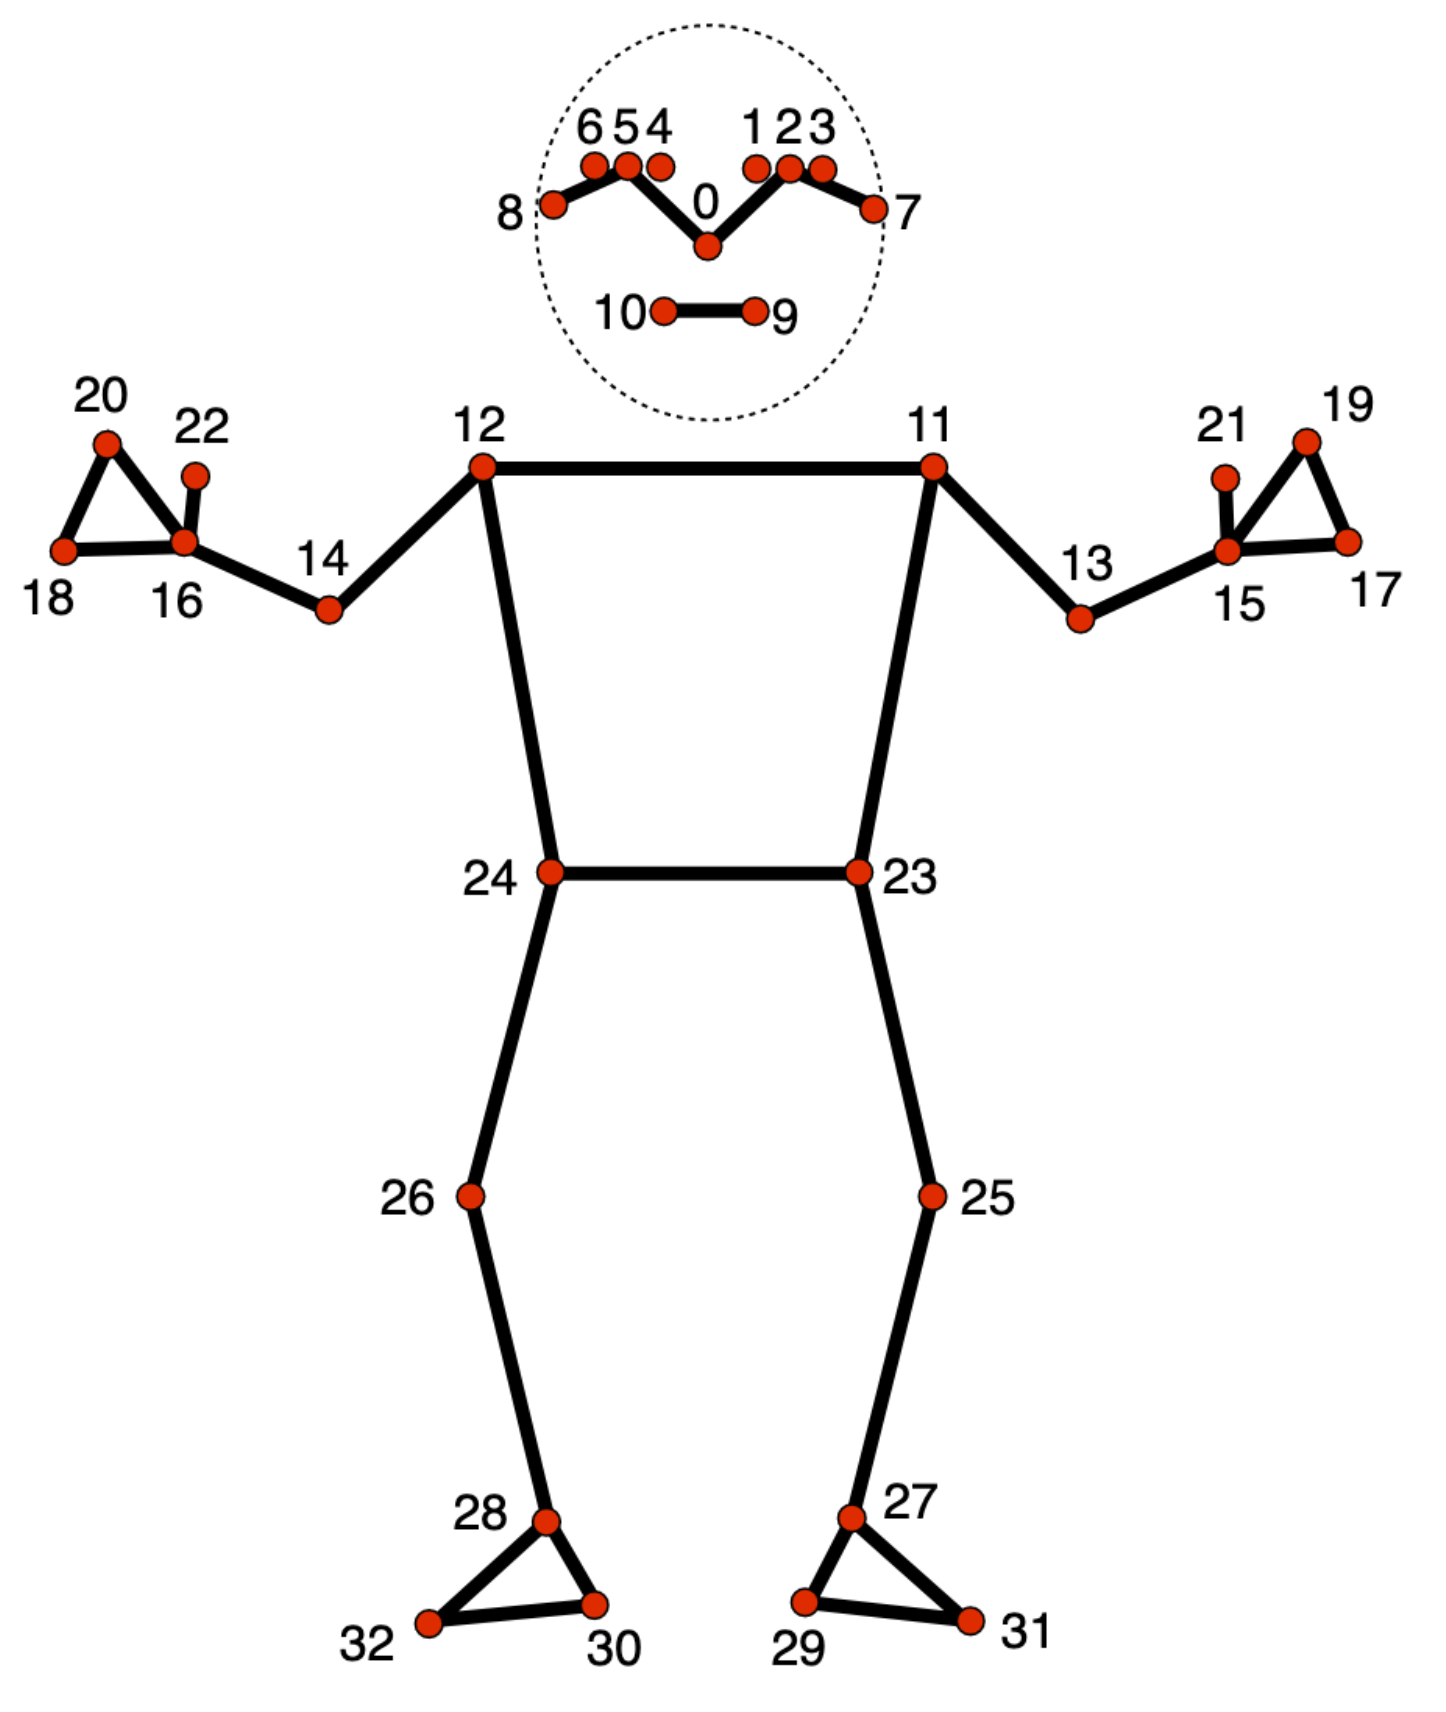
\includegraphics[height=0.8\textheight, keepaspectratio]{pose_landmarks_index.png}
        \vspace{0.2cm}
        {\small Keypoints cơ bản trong HPE (Human Pose Estimation).}
    \end{column}

    % Column Text
    \begin{column}{0.55\textwidth}
        \begin{block}{Khái niệm}
            Ước lượng vị trí khớp từ hình ảnh/video:
            \[
                \mathcal{K} = \{k_i = (x_i, y_i, z_i, c_i)\}
            \]
        \end{block}

        \begin{alertblock}{Phương pháp}
            \begin{itemize}
                \item \textbf{Top-down:} Phát hiện người trước, keypoints sau (MediaPipe)
                \item \textbf{Bottom-up:} Keypoints trước, nhóm sau (OpenPose)
            \end{itemize}
        \end{alertblock}
    \end{column}
\end{columns}
\end{frame}

% Slide 3: MediaPipe Pose

\begin{frame}{MediaPipe Pose Thời gian thực – Kiến trúc BlazePose}
    \begin{block}{Kiến trúc BlazePose}
        Tối ưu HPE 3D với:
        \begin{itemize}
            \item \textbf{Nodes:} Module xử lý.
            \item \textbf{Edges:} Luồng dữ liệu đồng bộ.
        \end{itemize}
    \end{block}
\end{frame}

\begin{frame}{MediaPipe Pose – Thành phần & Hậu xử lý}
    \begin{exampleblock}{Thành phần chính}
        \begin{itemize}
            \item \textbf{Detection:} ROI từ RGB.
            \item \textbf{Landmark:} 33 keypoints 3D, Loss: $\mathcal{L} = \sum \lambda_i \mathcal{L}_i$.
            \item \textbf{Tracking:} Dự đoán ROI.
        \end{itemize}
    \end{exampleblock}

    \begin{alertblock}{Hậu xử lý}
        \begin{itemize}
            \item One Euro Filter: Làm mịn nhiễu.
            \item Chuẩn hóa $z$: Dựa trên hông.
        \end{itemize}
    \end{alertblock}
\end{frame}

% Slide 4: Thuật toán Phát hiện Té ngã
\begin{frame}{Thuật toán Phát hiện Té ngã}
    \begin{columns}[t]
        \column{0.5\textwidth}
        \begin{block}{Đặc trưng Động học}
            \begin{itemize}
                \item Vận tốc: $\vec{v}_{\text{COM}} = \frac{\Delta \vec{p}}{\Delta t}$.
                \item Gia tốc: $a = \frac{\|\Delta \vec{v}\|}{\Delta t}$.
            \end{itemize}
        \end{block}
        \begin{block}{Đặc trưng Tư thế}
            \begin{itemize}
                \item \textbf{AR:} Tăng khi nằm ngang.
                \item \textbf{$\theta_{\text{body}}$:} Góc vai-hông.
                \item \textbf{$\Delta h_{\text{head}}$:} Giảm chiều cao.
            \end{itemize}
        \end{block}
        \column{0.5\textwidth}
        \begin{alertblock}{Ba Giai đoạn Phát hiện}
            \begin{enumerate}
                \item \textbf{Sớm:} Tốc độ/gia tốc COM cao.
                \item \textbf{Xác nhận:} AR, $\theta_{\text{body}}$ chỉ nằm ngang.
                \item \textbf{Bất động:} Chuyển động $< M_{th}$.
            \end{enumerate}
        \end{alertblock}
    \end{columns}
\end{frame}
